% !TEX root = recipeUnderstanding.tex

\vspace{-1mm}
\section{Forming the Multi-Modal Representation}
\label{atoms}
\vspace{-1mm}

Finding the set of activity steps over large collection of videos having large visual varieties requires us to represent the semantic information in addition to the low-level visual cues. Hence, we find our language and visual atoms by using mid-level cues like object proposals and frequent words.

\begin{figure}[h]
  \includegraphics[width=0.5\textwidth]{repr}
  \vspace{-8mm}
  \caption{We learn language and visual atoms to represent multi-modal information. Language atoms are frequent words and visual atoms are the clusters of object proposals.}
  \vspace{-3mm}
\label{fig:overview}
\end{figure}

\noindent\textbf{Learning Visual Atoms:} In order to learn visual atoms, we create a large collection of object proposals by independently generating object proposals from each frame of each video. These proposals are generated using the Constrained Parametric Min-Cut (CPMC) \cite{cpmc} algorithm based on both appearance and motion cues. We note the $k^{th}$ proposal of $t^{th}$ frame of $i^{th}$ video as $r^{(i),k}_t$. Moreover, we drop the video index $(i)$ if it is clearly implied in the context.

In order to group this object proposals into mid-level visual atoms, we follow a clustering approach. Although any graph clustering approach (\eg, Keysegments \cite{keysegments}) can be applied for this, the joint processing of a large video collection requires handling large visual variability among multiple videos. We propose a new method to jointly cluster object proposals over multiple videos in Section~\ref{jointProp}. Each cluster of object proposals correspond to a visual atom.

\noindent\textbf{Learning Language Atoms:}
We define the language atoms as the salient words which occur more often than their ordinary rates based on the \emph{tf-idf} measure. The \emph{document} is defined as the concatenation of all subtitles of all frames of all videos in the collection as $D=\bigcup_{i \in N_C} \bigcup_{t \in T^{(i)}} L_t^i$. Then, we follow the classical tf-idf measure and use it as $tfidf(w,D)=f_{w,D} \times \log \left( 1+ \frac{N}{n_{w}}\right)$ where $w$ is the word we are computing the tf-idf score for, $f_{w,D}$ is the frequency of the word in the \emph{document} $D$, $N$ is the total number of video collections we are processing, and $n_{w}$ is the number of video collections whose subtitle include the word $w$.

We sort words with their ``tf-idf" values and choose the top $K$ words as language atoms (\emph{$K=100$ in our experiments}). As an example, we show the language atoms learned for the category \emph{making scrambled egg} in Figure~\ref{fig:overview}. %The resulting collection suggests that they correspond to the important objects, actions and adjectives which represent a semantic information occurring over multiple videos.

%\begin{figure}
%\footnotesize
%\emph{sort, place, water, egg, bottom, fresh, pot, crack, cold, cover, time, overcooking, hot, shell, stove, turn, cook, boil, break, pinch, salt, peel, lid, point, high, rules, perfectly, hard, smell, fast, soft, chill, ice, bowl, remove, aside, store, set, temperature, coagulates, yolk, drain, swirl, shake, white, roll, handle, surface, flat}
%\normalsize
%\caption{Language atoms learned for activity class \emph{"How to hard boil an egg?"}}
%\end{figure}

\noindent\textbf{Representing Frames with Atoms:}
After learning the visual and language atoms, we represent each frame via the occurrence of atoms (binary histogram). Formally, the representation of the $t^{th}$ frame of the $i^{th}$ video is denoted as $\mathbf{y^{(i)}_t}$ and computed as $\mathbf{y^{(i)}_t}=[\mathbf{y^{(i),l}_t},\mathbf{y^{(i),v}_t}]$ such that $k^{th}$ entry of the $\mathbf{y^{(i),l}_t}$ is $1$ if the subtitle of the frame has the $k^{th}$ language atom and $0$ otherwise. $\mathbf{y^{(i),v}_t}$ is also a binary vector similarly defined over visual atoms. We visualize the representation of a sample frame in the Figure~\ref{visFrame}.
\begin{figure}[h!]
  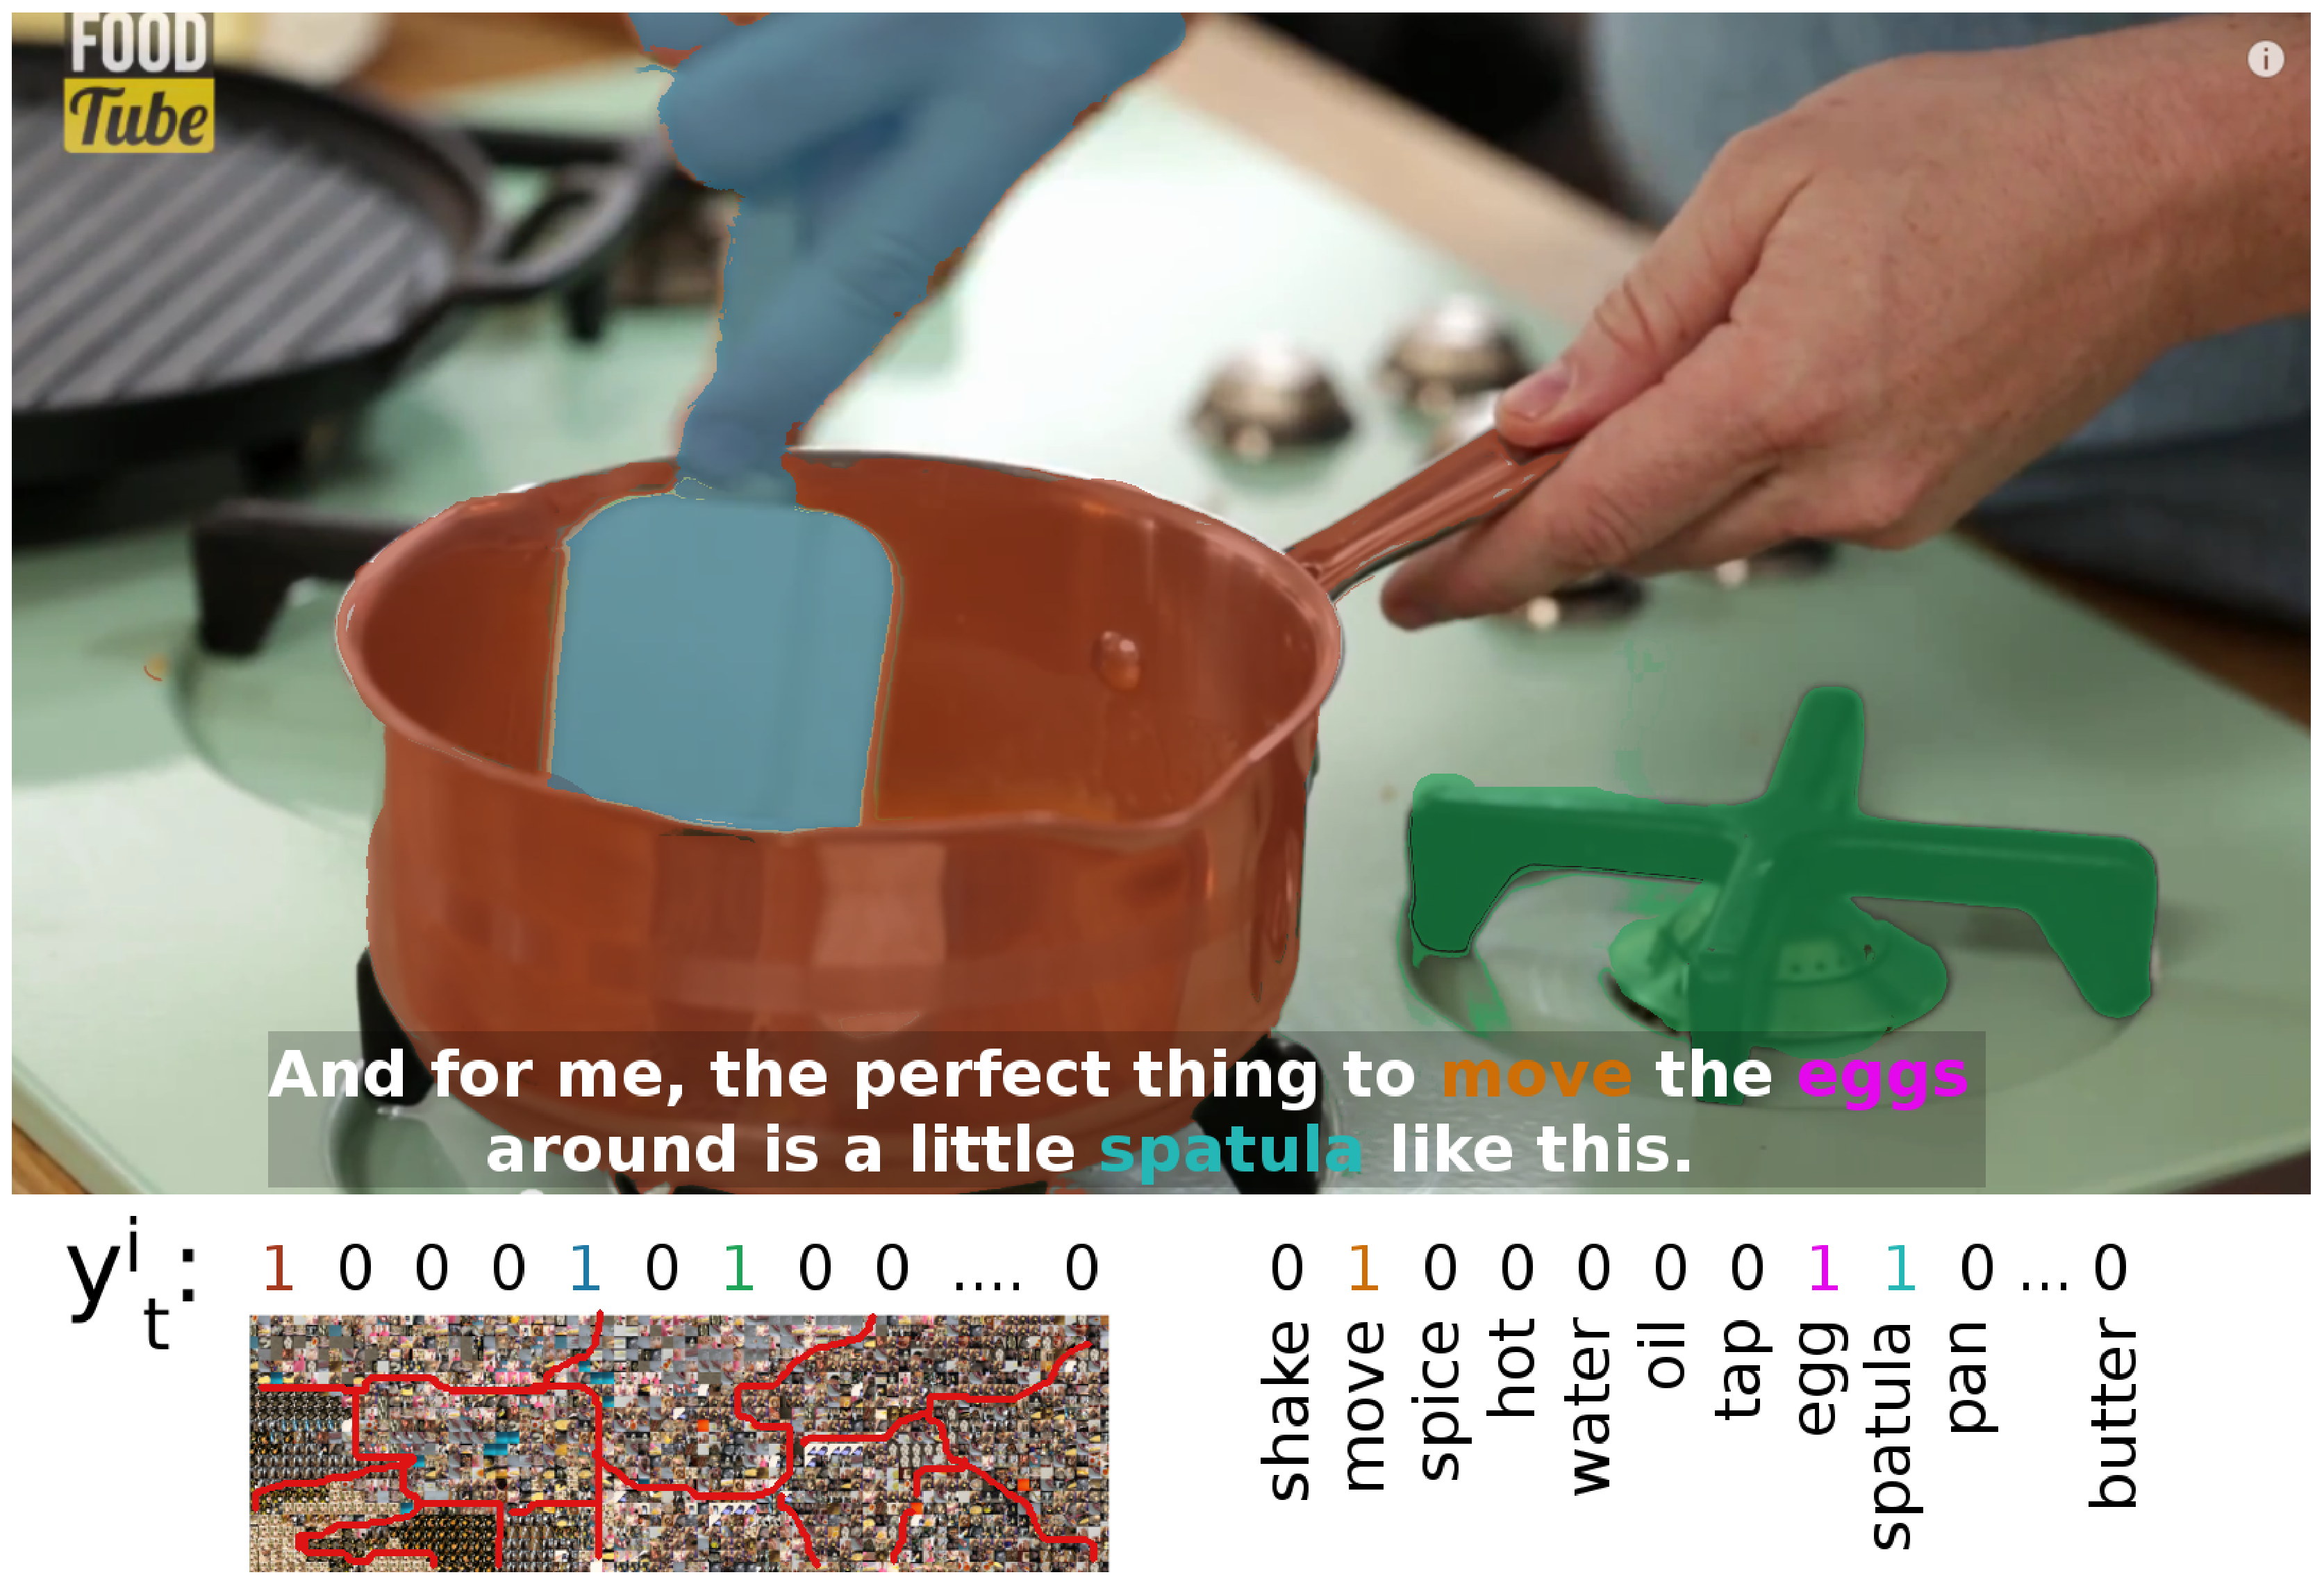
\includegraphics[width=0.46\textwidth]{frame}
%    \vspace{-1mm}
  \caption{\textbf{Representation for a sample frame.} Three of the object proposals of sample frame are in the visual atoms and three of the words are in the language atoms.}
  \label{visFrame}
  \vspace{-4mm}
\end{figure}

\vspace{-1mm}
\section{Joint Proposal Clustering over Videos}
\label{jointProp}
\vspace{-1mm}

Given a set of object proposals generated from ``multiple videos", simply combining them into a single collection and clustering them into atoms is not desirable for two reasons: (1) semantic concepts have large visual differences among different videos and accurately clustering them into a single atom is hard, (2) atoms should contain object proposals from multiple videos in order to semantically relate the videos. In order to satisfy these requirements, we propose a joint extension to spectral clustering. Note that the purpose of this clustering is generating atoms where each clusters represents an atom.

\begin{figure}[ht]
  \includegraphics[width=0.48\textwidth]{joint_clustering}
  %\scalebox{0.85}{
%  $\arg\max  \frac{x_1^TA^{(1)}x^1}{x_1^Tx^1}+\frac{x_2^TA^{(2)}x^2}{x_2^Tx^2}+\frac{x_3^TA^{(3)}x^3}{x_3^Tx^3}+\frac{x_1^TA^{(1,2)}x^2}{x_1^T\mathds{1}\mathds{1}^Tx^2}+\frac{x_2^TA^{(2,3)}x^3}{x_2^T\mathds{1}\mathds{1}^Tx^3}$}
  %$\arg\max  \color[HTML]{BF9000}{\frac{x_1^TA^{(1)}x^1}{x_1^Tx^1}}+\color[HTML]{990000}{\frac{x_2^TA^{(2)}x^2}{x_2^Tx^2}}+\color[HTML]{38761d}{\frac{x_3^TA^{(3)}x^3}{x_3^Tx^3}}+\color[HTML]{a64d79}{\frac{x_1^TA^{(1,2)}x^2}{x_1^T\mathds{1}\mathds{1}^Tx^2}}+\color[HTML]{F1C232}{\frac{x_2^TA^{(2,3)}x^3}{x_2^T\mathds{1}\mathds{1}^Tx^3}}$}
  \vskip -2mm
\caption{\textbf{Joint proposal clustering.} Here, we show the $1^{st}NN$ video graph and $2^{nd}NN$ region graph. Each object proposal is linked to its two NNs from the video it belongs and two NNs from the videos it is neighbour of. Black nodes are the proposals selected as part of the cluster and the gray ones are not selected. Moreover, dashed lines are intra-video edges and solid ones are inter-video edges.}
  \label{hierProposal}
    \vskip -1mm
\end{figure}

\noindent\textbf{Basic Graph Clustering:} Consider the set of object proposals extracted from a single video $\{r^k_t\}$, and a pairwise similarity metric $d(\cdot,\cdot)$ for them. We follow the single cluster graph partitioning (SCGP)\cite{scgp} approach to find the dominant cluster which maximizes the intra-cluster similarity:
\begin{equation}
  \argmax_{x^k_t} \frac{\sum_{(k_1,t_1),(k_2,t_2) \in K \times T} x^{k_1}_{t_1} x^{k_2}_{t_2} d(r^{k_1}_{t_1},r^{k_2}_{t_2})}{\sum_{(k,t) \in K \times T} x^{k}_t}
  \label{nonvec}
\end{equation}
where $x^{k}_t$ is a binary variable which is $1$ if $r^{k}_t$ is included in the cluster, $T$ is the number of frames and $K$ is the number of clusters per frame. Adopting the vector form of the indicator variables as $\mathbf{x_{tK+k}}=x^{k}_{t}$ and the pairwise distance matrix as $\mathbf{A}_{t_1K+k_1,t_2K+k_2}=d(r^{k_1}_{t_1},r^{k_2}_{t_2})$, equation (\ref{nonvec}) can be compactly written as
$\argmax_{\mathbf{x}} \frac{\mathbf{x^T}A\mathbf{x}}{\mathbf{x^T}\mathbf{x}}$
This can be solved by finding the dominant eigenvector of $\mathbf{x}$ after relaxing $x^{k}_t$ to $[0,1]$ \cite{scgp,scgp_eigen}. Upon finding the cluster, the members of the selected cluster are removed from the collection and the same algorithm is applied to find remaining clusters.

\noindent\textbf{Joint Clustering:} Our extension of the SCGP into multiple videos is based on the assumption that the key objects occur in most of the videos. Hence, we re-formulate the problem by enforcing the homogeneity of the cluster over all videos.

We first create a kNN graph of the videos based on the distance between their textual descriptions. We use the $\chi^2$ distance of the bag-of-words computed from the video description. We also create the kNN graph of object proposals in each video based on the pretrained "fc7" features of AlexNet~\cite{alexnet}. This hierarchical graph structure is visualized in Figure~\ref{hierProposal} for three videos samples. After creating this graph, we impose both ``inter-video" and ``intra-video" similarity among the object proposals of each cluster. Main rationale behind this construction is having a separate notion of distance for inter-video and intra-video relations since the visual similarity decreases drastically for inter-video ones.

Given the intra-video distance matrices $\mathbf{A^{(i)}}$, the binary indicator vectors $\mathbf{x^{(i)}}$, and the inter-video distance matrices as $\mathbf{A^{(i,j)}}$, we define our optimization problem as;
\begin{equation}
\argmax \sum_{i \in N} \frac{\mathbf{x^{(i)^T}}\mathbf{A^{(i)}}\mathbf{x^{(i)}}}{\mathbf{x^{(i)^T}}\mathbf{x^{(i)}}} +
\sum_{i \in N} \sum_{j \in \mathcal{N}(i)} \frac{\mathbf{x^{(i)^T}}\mathbf{A^{(i,j)}}\mathbf{x^{(j)}}} {\mathbf{x^{(i)^T}}\mathds{1}\mathds{1}^T\mathbf{x^{(j)}}},
\end{equation}
where $\mathcal{N}(i)$ is the neighbours of the video $i$ in the kNN graph, $\mathds{1}$ is vector of ones and $N$ is the number of videos.

Although we can not use the efficient eigen-decomposition approach from \cite{scgp,scgp_eigen} as a result of the modification, we can use Stochastic Gradient Descent as the cost function is quasi-convex when relaxed. We use the SGD with the following analytic gradient function:
\begin{equation}
  \nabla_{\mathbf{x^{(i)}}} = \frac{2\mathbf{A^{(i)}} \mathbf{x^{(i)}} -2\mathbf{x^{(i)}} r^{(i)}}
  {\mathbf{{x^{(i)}}^T}\mathbf{x^{(i)}}}
+ \sum_{i \in N} \frac{\mathbf{A^{i,j}}\mathbf{x^{j}} - \mathbf{{x^{(j)}}^T} \mathds{1} r^{(i,j)}}{\mathbf{{x^{(i)}}^T} \mathds{1} \mathds{1}^T \mathbf{x^{(j)}} },
  %\text{Some vector matrix multiplication}
\end{equation}
where $r^{(i)}=\frac{\mathbf{x^{(i)^T}}\mathbf{A^{(i)}}\mathbf{x^{(i)}}}{\mathbf{x^{(i)^T}}\mathbf{x^{(i)}}}$ and $r^{(i,j)}=\frac{\mathbf{x^{(i)^T}}\mathbf{A^{(i,j)}}\mathbf{x^{(j)}}} {\mathbf{x^{(i)^T}}\mathds{1}\mathds{1}^T\mathbf{x^{(j)}}}$

We iteratively use the method to find clusters, and stop after the $K=20$ clusters are found as the remaining object proposals were deemed not relevant to the activity. Each cluster corresponds to a visual atom for our application.

In Figure~\ref{cvis}, we visualize some of the atoms (\ie, clusters) we learned for the query \emph{How to Hard Boil an Egg?}. As apparent in the figure, the resulting atoms are highly correlated and correspond to semantic objects\&concepts regardless of their significant intra-class variability.
\begin{figure}[ht]
  \begin{subfigure}[b]{0.23\textwidth}
\includegraphics[width=\textwidth]{im0.png}
%\caption{Cluster 1}
\end{subfigure}
~
\begin{subfigure}[b]{0.23\textwidth}
\includegraphics[width=\textwidth]{im4.png}
%\caption{Cluster 2}
\end{subfigure}

%\begin{subfigure}[b]{0.23\textwidth}
%\includegraphics[width=\textwidth]{im5.png}
%\end{subfigure}
%~
%\begin{subfigure}[b]{0.23\textwidth}
%\includegraphics[width=\textwidth]{im7.png}
%\end{subfigure}

\begin{subfigure}[b]{0.23\textwidth}
\includegraphics[width=\textwidth]{im8.png}
\end{subfigure}
~
\begin{subfigure}[b]{0.23\textwidth}
\includegraphics[width=\textwidth]{im10.png}
\end{subfigure}
%\vspace{-1mm}
\caption{Randomly selected images of four randomly selected clusters learned for \emph{How to hard boil an egg?}}
\label{cvis}
\vspace{-3mm}
\end{figure}
